\newenvironment{slots}
{%
  \begin{flushleft}%
    \tablehead{}%
    \begin{supertabular}{|m{2.8669999cm}|m{12.472cm}|}%
      \hline%
      \bfseries Slot &%
      \bfseries Description\\\hline%
    }
    {%
    \end{supertabular}%
  \end{flushleft}%
}


\section{Introduction}

This document aims at clarifying the naming conventions
in URBI Engines for standard hardware/software devices and components
implemented as UObject and the corresponding
methods/attributes/events to access them. The list of available
hardware types and software component is increasing and this document
will be updated accordingly. Please contact us directly, should you be
working on a component not described or closely related to one
described here:

{\centering\itshape
standard@gostai.com
\par}


Any implementation of an URBI server must comply with the latest version
of this standard to get the ``URBI ready''
certification from Gostai S.A.S.


Gostai S.A.S. is currently the only authority which has the ability to
deliver an ``URBI Ready'' certification.

{
“URBI Ready” and the associated logo are trademarks of Gostai S.A.S. and
should not be used or displayed in any way without an explicit written
agreement from Gostai.}

\section{The Structure Tree}

The robot will be described as a set of
\textit{components} organized in a hierarchical
structure called the \textit{structure tree}. The
relationship between a component and a sub-component in the tree is a
‘part-of’ inclusion relationship. From the point of view of URBI, each
component in the tree is an object, and it contains attributes pointing
to its sub-components. Here is a example illustrating a part of a
hierarchy that could be found with a humanoid robot:



\begin{figure}
\centering
%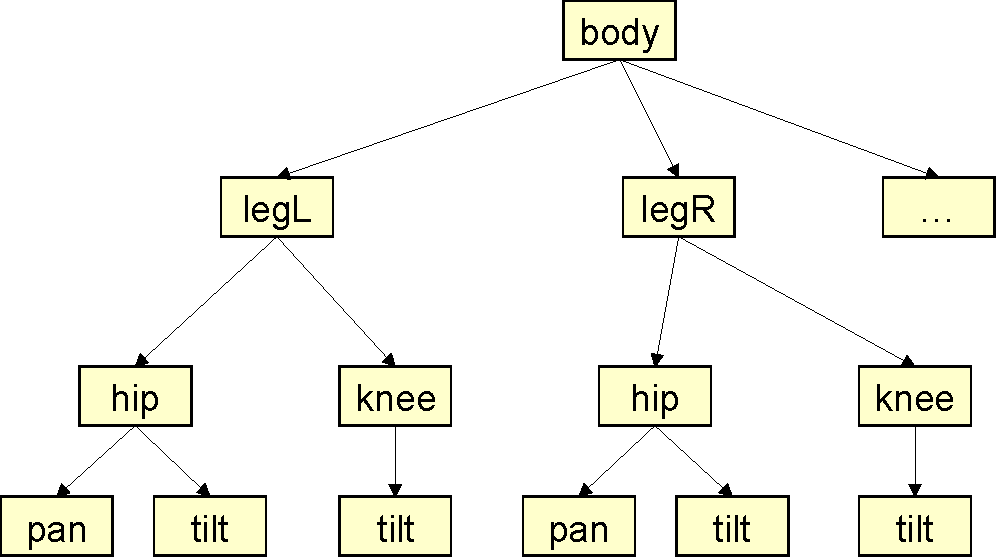
\includegraphics[width=10.146cm,height=5.683cm]{namingstandard-img/namingstandard-img3.pdf}
\end{figure}

The leaves of the tree are called
\textit{devices}, and they usually match physical
devices in the robot: motors, sensors, lights, camera, etc. Inside
URBI, the various objects corresponding to the tree components are
accessed by following the path of objects inclusions, like in the
example below (shortcuts will be described later):

{
body.legR.hip.tilt}

{
body.legL.knee.led}

{
body.legL.hip}

{
…}


The structure tree should not be mistaken for a representation of the
kinematics chain of the robot. The kinematics chain is built from a
subset of the devices corresponding to motor devices, and it represents
spatial connections between them. Except for these motor devices, the
structure tree components do not have a direct counterpart in the
kinematics chain, or, if they do, it is as a subset of the kinematics
chain (for example, \texttt{legR} is a subset of the whole kinematics
chain).


The goal of this standard is to provide guidelines on how to define the
components and the structure tree, knowing the kinematics chain of the
robot.

\section{Frame of Reference}

In many cases, it will be necessary to refer to an absolute frame of
reference attached to the robot body. To avoid ambiguities, the
standard frame of reference will have the following definition:

\begin{figure}
\centering
 [Warning: Image ignored] % Unhandled or unsupported graphics:
%%\includegraphics[width=7.458cm,height=7.1cm]{}

\end{figure}

\begin{description}
\item[Origin] the center of mass of the robot
\item[X axis] oriented towards the front of the
robot. If there is a camera, the front is defined by the default
direction of the camera, otherwise the front will be seen as the
natural frontal orientation for a mobile robot (the direction of
“forward” movement). If the robot is not naturally oriented, the X axis
will be chosen to match the main axis of symmetry of the robot body and
it will be oriented towards the smallest side, typically the top of a
cone for example. In case of a perfectly symmetrical body, the
X axis can be chosen arbitrarily but a clear mark should be made
visible on the robot body to indicate it.
\item[Z axis] oriented in the opposite direction
from the gravity. If there is no gravity or natural up/down orientation
in the environment or normal operation mode of the robot, the Z axis
should be chosen in the direction of the main axis of symmetry in the
orthogonal plane defined by the X axis, oriented towards the smallest
side. In case of a perfectly symmetrical plane, the Z axis can be
chosen arbitrarily but a clear mark should be made visible on the robot
body to indicate it.
\item[Y axis] oriented to make a right-handed
coordinate system.
\end{description}


The axes are oriented in a counter-clockwise direction, as depicted in
the illustration above.

\section{Component naming}

The name of a component A, which is a sub-component of component
B, is divided into two parts: the generic designation of a subpart of
the kinematics chain (like ‘leg’, ‘head’, ‘finger’) that A is referring
to, and optionally some topological disambiguator relative to its
position within the component B it belongs to. For example, when there
are two legs, we need to differentiate between the right and left leg,
relative to the body component they belong to. The first part is called
the \textit{designation}, and the second optional
part is called the \textit{localization}.

\paragraph{Designation}


The designation of a component is a usually robot-specific and depends
on the class of the robot (wheeled, humanoid, animaloid, etc). We will
give in the following chapters some guidelines for the most current
designations, and we will give more advanced rules for rare customized
cases.


The designation is the critical part of the naming standard. We cannot
possibly cover all future configurations and conceivable robot complex
bodies, but the current document will grow whenever we find a new case.
We hope to be already covering most of the main cases you can find in
the industry.

\paragraph{Localization }

Localization is necessary when there are two identical
sub-components A1 and A2 belonging to the same component B, like for
example two legs or two arms attached to the main body. Usually this
can be sorted out with simple geometric qualifiers like
\textit{Right/Center/Left},
\textit{Front/Middle/Back} or
\textit{Up}\textit{/In-between/Down}. The
naming convention is to use the first letter of the geometric
characteristic, like R for Right, I for In-between.
Note that “right” or “front” are understood here from the point of view
of a man standing and looking in the direction of the X-axis of the
robot, and
\textit{Up}/\textit{Down} matches
the Z-axis, as depicted in the figure below:

{\centering [Warning: Draw object ignored][Warning: Draw object
ignored]\par}

Several geometric qualifiers can be used at the same time to
further refine the position. As a convention, side information comes
first (R/C/L), followed by the depth
information (F/M/H) and then the height
information (U/I/D).


You can further qualify a side+depth localization with an additional R/L
side information. This can be used in the typical layout below:

{\centering
%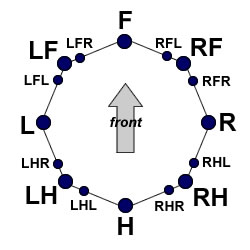
\includegraphics[width=8.819cm,height=8.819cm]{namingstandard-img/namingstandard-img4.jpg}
\par}


This dual positioning using side+depth can also be used to combine
side+height or height+depth information.


Some layouts will typically imply a bilateral organization like for
example an insectoid robot with a series of 3 legs on both side of its
body. In that case, an array will be used and follow the geometrical
localization (R/L). The smaller the number, the closer to the front:
R[1], R[2], R[3] and L[1], L[2], L[3]. This can be used when there is
at least 3 components on each side, otherwise the
\textit{Front}/\textit{Back} approach prevails.


Some components like spines or tails are highly articulated with a set
of identical sub-components. When talking about these sub-components,
the above localization should be replaced by an array with a numbering
starting at 0. The smaller the number, the closer the sub-component is
to the robot main body. For surface-like sub-components, like skin
touch sensors, the array can be two dimensional.


Other possible localization for sensors are the X, Y and Z axis
themselves, like for example for an accelerometer or a gyro sensor,
available in each of the three directions.


Examples of component names including localization:

{
legR, legL, armR, armL}

{
fingerR, fingerC, fingerL // three fingers hand}

{
joint[0], joint[1] … joint[5] // from tail}

{
touch[478][124] // from skin}

{
accelX, accelY, accelZ // typical accelerometer}

{
gyroX, gyroY, gyroZ // tpycial gyro sensor}

\section{Facets}

URBI allows multiple inheritances between objects. This feature can be
used to introduce the notion of “facet”. A facet is an object in URBI
that describes some aspect of a type of component.


For example, for a joint, we can have a “swivel” facet, used to define
patella joints. For the robot body itself, we have a “mobile” facet
describing mobile robots, which includes some standard way of
requesting a move forward, a turn, etc. A robot with a Pan/Tilt camera
or otherwise moving camera will have the “panoramic” facet which is
abstracting the way the robot can turn its gaze in any direction.


In short, facets are standard Urbi objects that components can inherit
from to acquire some functionalities, expressed as a standard
interface. We will describe in the following pages a few of the most
standard facets. Each facet should be reimplemented for any particular
robot that uses them, for example the “mobile” facet will have a
completely different implementation with a humanoid robot and a wheeled
robot.

\paragraph{identity}


Contains information about the robot identity.

\subparagraph{Slots}

\begin{slots}
type &
This describes the robot category
among: humanoid, fourlegged, wheeled, industrial arm. It gives a
general idea of the robot family, but does not replace a more
systematic probe of available services by investigating the list of
attributes of the object.\\\hline
name &
Name of the robot.\\\hline
model &
Model of the robot.\\\hline
serial &
Serial number (if available).\\\hline
\end{slots}


\paragraph{network}

Contains information about the network identification of the robot.

\subparagraph{Slots}

\begin{slots}
IP &
IP address of the robot.\\\hline
gateway &
Gateway IP address.\\\hline
latency &
Measured average network
latency.\\\hline
bandwidth &
Measured average network
bandwidth.\\\hline
\end{slots}

\paragraph{motor}

This facet is used to describe a generic motor controller.

\subparagraph{Slots}

\begin{slots}
val &
This slot is a generic pointer to a
more specific slot describing the motor position, like
\texttt{position} or \texttt{angle}, depending on the type of motor. It
is mandatory in the Urbi Ready standard as a universal proxy to control
an actuator. The more specific slot is described in a subclass of
\texttt{motor}.\\\hline
PGain &
Controls the P gain of the PID
controller.\\\hline
IGain &
Controls the I gain of the PID
controller.\\\hline
DGain &
Controls the D gain of the PID
controller.\\\hline
\end{slots}


\begin{flushleft}
\tablehead{}
\begin{supertabular}{|m{1.717cm}|m{10.464cm}}
\hhline{-~}
 &
Optional slot.\\\hhline{-~}
\end{supertabular}
\end{flushleft}
\paragraph{ linearMotor  \textmd{subclass of motor}}


This facet is used to describe a linear motor controller.

\subparagraph{Slots}

\begin{slots}
position &
Position of the motor in centimeters.
Pointed to by the \texttt{val} slot.\\\hline
force &
Intensity of the measured or estimated
force applied on a linear motor.\\\hline
\end{slots}
{
     \textbf{\textit{rotationalMotor}}
\textit{subclass of motor}}


This facet is used to describe a rotational motor controller.

\subparagraph{Slots}

\begin{slots}
angle &
Angle of the motor in degree, modulo
360. Pointed to by the \texttt{val} slot.\\\hline
turn &
Absolute angular position of the
motor, expressed in number of turns.\\\hline
torque &
Intensity of the measured or estimated
torque applied on the motor.\\\hline
\end{slots}


\paragraph{sensor}

This facet is used to describe a generic sensor.

\subparagraph{Slots}

\begin{slots}
val &
This slot is a generic pointer to a
more specific slot describing the sensor value, like \texttt{distance}
or \texttt{temperature}, depending on the type of sensor. It is
mandatory in the Urbi Ready standard as a universal proxy to read a
sensor. The more specific slot is described in a subclass of
\texttt{sensor}.\\\hline
\end{slots}


\paragraph{ distanceSensor  \textmd{subclass of sensor}}

This facet is used to describe a distance sensor (infrared, laser,
ultrasonic...).

\subparagraph{Slots}

\begin{slots}
distance &
Measured distance expressed in meters.
Pointed to by the \texttt{val} slot.\\\hline
\end{slots}


\paragraph{ touchSensor  \textmd{subclass of sensor}}

This facet is used to describe a touch pressure sensor (contact,
induction,...).

\subparagraph{Slots}

\begin{slots}
pressure &
Intensity of the pressure put on the
touch sensor. Can be 0/1 for simple buttons or expressed in Pascal
units. Pointed to by the \texttt{val} slot.\\\hline
\end{slots}


\paragraph{ accelerationSensor  \textmd{subclass of sensor}}

This facet is used to describe an accelerometer.

\subparagraph{Slots}

\begin{slots}
acceleration &
Acceleration expressed in m/s2.
Pointed to by the \texttt{val} slot.\\\hline
\end{slots}

\paragraph{gyroSensor  \textmd{subclass of sensor}}

This facet is used to describe an gyrometer.

\subparagraph{Slots}

\begin{slots}
acceleration &
Acceleration expressed in rad/s2.
Pointed to by the \texttt{val} slot.\\\hline
\end{slots}

\paragraph{ temperatureSensor  \textmd{subclass of sensor}}


This facet is used to describe a temperature sensor.

\subparagraph{Slots}

\begin{slots}
temperature &
Measured temperature in Celsius degrees.
Pointed to by the \texttt{val} slot.\\\hline
\end{slots}

\paragraph{mobile}

Mobile robots all share this generic interface to provide high order
level motion control capabilities.

\subparagraph{Slots}

\begin{slots}
go(x) &
Move approximatively x meters forward
if x is positive, backward otherwise.\\\hline
turn(x) &
Turn right approximatively x degrees.
x can be a positive or negative value.\\\hline
\end{slots}

\paragraph{tracker}

Camera-equipped robots can sometimes move the orientation of the field
of view horizontally and vertically, which is a very important feature
for many applications. In that case, this facet abstracts how such
motion can be achieved, whether it is done with a pan/tilt camera or
with whole body motion or a combination of both.

\subparagraph{Slots}

\begin{slots}
yaw &
Rotational articulation around the Z
axis in the robot, expressed in degrees.\\\hline
pitch &
Rotational articulation around the Y
axis in the robot, expressed in degrees.\\\hline
\end{slots}

\paragraph{videoin}

The videoin facet groups every information relative to cameras or any
image sensor.

\subparagraph{Slots}

\begin{slots}
val &
Binary value corresponding to the
image, expressed in the current unit (RGB, jpeg, YCrCb...). The unit
can be changed like any other regular unit in Urbi. \\\hline
xfov &
The x Field Of View of the camera
expressed in degrees.\\\hline
yfov &
The y Field Of View of the camera
expressed in degrees.\\\hline
height &
Height of the image in the current
resolution, expressed in pixels\\\hline
width &
Width of the image in the current
resolution, expressed in pixels\\\hline
shutter &
The shutter speed (expressed
in ms). 0 if non applicable.\\\hline
wb &
White balance (expressed with
an integer value depending on the camera documentation). 0 if non
applicable.\\\hline
gain &
Camera gain amplification
(expressed as a coefficient between 0 and infinity). 1 if non
applicable.\\\hline
resolution &
 Can be used to specify a given
resolution, expressed as a percentage of the maximal resolution of the
camera (number between 0 and 1). 1 if non applicable.

Once modified, the effective
resolution in X/Y can be checked with the width and height
slots.\\\hline
\end{slots}

\begin{flushleft}
\tablehead{}
\begin{supertabular}{|m{1.717cm}|m{10.464cm}}
\hhline{-~}
 &
Optional slot.\\\hhline{-~}
\end{supertabular}
\end{flushleft}
\paragraph{audioout}


The audioout facet groups every information relative to speakers.

\subparagraph{Slots}

\begin{slots}
val &
 The speaker value, expressed as a
binary, in the format given by the binary header during the
assignment.

Speakers are write-only devices, so
there is not much sense in reading the content of this attribute. At
best, it returns the remaining sound to be played if it is not over
yet, but this is not a requirement.\\\hline
remain &
The amount of time remaining to play in
the speaker sound buffer (expressed in \textit{ms} as
a default unit).\\\hline
playing &
This is a boolean value which is true
when there is a sound currently playing (the buffer is not
empty)\\\hline
volume &
Volume of the play back, in
decibels.\\\hline
\end{slots}

\begin{flushleft}
\tablehead{}
\begin{supertabular}{|m{1.717cm}|m{10.464cm}}
\hhline{-~}
 &
Optional slot.\\\hhline{-~}
\end{supertabular}
\end{flushleft}


\paragraph{audioin}

The audioin facet groups every information relative to microphones.

\subparagraph{Slots}

\begin{slots}
val &
 Binary value corresponding to the
sound heard, expressed in the current unit (wav, mp3...). The unit can
be changed like any other regular unit in Urbi.

The content is the sound heard by the
microphone since the last update event.\\\hline
duration &
Amount of sound in the val
attribute, expressed in \textit{ms}.\\\hline
gain &
Microphone gain amplification
(expressed between 0 and 1)\\\hline
\end{slots}

\begin{flushleft}
\tablehead{}
\begin{supertabular}{|m{1.717cm}|m{10.464cm}}
\hhline{-~}
 &
Optional slot.\\\hhline{-~}
\end{supertabular}
\end{flushleft}


\paragraph{blobDetector}

Ball detectors, marker detectors and various feature-based detectors
should all share a similar interface. They extract a part of the image
that fits some criteria and define a “blob” accordingly. Here are the
typical slots expected:

\subparagraph{Slots}

\begin{slots}
x &
The x position of the center of the
blob in the image\\\hline
y &
The y position of the center of the
blob in the image\\\hline
ratio &
The size of the blob expressed as a
normalized image size: 1 = full image, 0 = nothing.\\\hline
visible &
A Boolean expressing whether there is a
blob in the image or not (see threshold)\\\hline
threshold &
The minimum value of ratio to
decide that the blob is visible.\\\hline
orientation &
Angle of the main ellipsoid axis of
the blog (0 = horizontal), expressed in degrees.\\\hline
elongation &
Ratio between the main and the second
diameter of the blob enveloping ellipse.\\\hline
\end{slots}

\begin{flushleft}
\tablehead{}
\begin{supertabular}{|m{1.717cm}|m{10.464cm}}
\hhline{-~}
 &
Optional slot.\\\hhline{-~}
\end{supertabular}
\end{flushleft}
\paragraph{textToSpeech}


Text to speech allows to read text using a speech synthetizor. Default
implementations should use the \texttt{speaker} component (or alias) as
their default sound output.

\subparagraph{Slots}

\begin{slots}
lang &
The language used, in international
notation (fr, en, it…): ISO 639\\\hline
speed &
How fast the voice should go, between
0 and 1.\\\hline
pitch &
Voice pitch, between 0 and 1.\\\hline
gender &
Gender of the speaker
(0:male/1:female)\\\hline
age &
Age of the speaker, if
applicable\\\hline
name &
Most TTS engine will propose several
voices, this attributes allows picking one. It’s a string identifier
specific to the TTS developer.\\\hline
say(s) &
Speak the sentence given in parameter
\var{s}.\\\hline
voicexml(s) &
Speak the text
\var{s} expressed as a VoiceXML
string.\\\hline
script(s) &
Speak the text
\var{s} augmented by script markups (see
specific Gostai documentation) to generate URBI events.\\\hline
\end{slots}

\begin{flushleft}
\tablehead{}
\begin{supertabular}{|m{1.717cm}|m{10.464cm}}
\hhline{-~}
 &
Optional slot.\\\hhline{-~}
\end{supertabular}
\end{flushleft}


\paragraph{speechRecognizer}

Speech recognition allows to transform a stream of sound into a text
using various speech recognition algorithms. Default implementations
should use the \texttt{micro} component (or alias) as their default
sound input.

\subparagraph{Slots}

\begin{slots}
lang &
The language used, in international
notation (fr, en, it…): ISO 639\\\hline
\end{slots}

\begin{flushleft}
\tablehead{}
\begin{supertabular}{|m{1.717cm}|m{10.464cm}}
\hhline{-~}
 &
Optional slot.\\\hhline{-~}
\end{supertabular}
\end{flushleft}
\subparagraph{Events}

\begin{slots}
hear(s) &
This event has one parameter which is
the string describing what the speech engine has recognized (can be a
word or a sentence).\\\hline
\end{slots}
\section{Standard Components}

Standard components correspond to components typically found in wheeled
robots, humanoid or animaloid robots, or in industrial arms.


The table on the next pages summarize the currently referenced standard
components, with a description of potential components that they could
be subcomponent of, a description of potential components they may
contain, and a list of relevant facets. This table should be seen as a
quick reference guide to identify available components in a given
robot.

\paragraph{Yaw/Pitch/Roll orientation: guideline}


It is not always clear which rotational direction corresponds to the
yaw, pitch or roll components (listed in the table below). This is a
quick guideline to help determine the proper association.


Let us consider the robot in its resting, most prototypical position,
like “standing” on two or four legs for a humanoid or animaloid, and
let all members “naturally” fall under gravity. When gravity has no
effect on a certain joint (because it is in the orthogonal plan to Z,
for example), the medium position between rangemin and rangemax should
be used. The body position achieved will be considered as a reference.
Then for each component that is described in terms of yaw/pitch/roll
sub-decomposition, the association will be as follow:

{
\textbf{ yaw} : rotational articulation around the Z
axis in the robot.}


\textbf{ pitch} : rotational articulation around the Y axis in the
robot.


\textbf{ roll} : rotational articulation around the X axis in the
robot.


When there is no exact match with the X/Y/Z axis, the closest match, or
the default remaining available axis, should be selected to determine
the yaw/pitch/roll meaning.

\begin{center}
\tablehead{\hline
\bfseries Component &
\bfseries Description &
\bfseries Sub. of &
\bfseries Contains &
\bfseries Facets\\\hline}
\begin{supertabular}{|m{2.312cm}|m{6.776cm}|m{2.629cm}|m{2.471cm}|m{2.1269999cm}|}
robot &
This is the main component that
represents an abstraction of the robot. &
\ttfamily {}- &
\ttfamily body &
\ttfamily identity network mobile
tracker\\\hline
body &
This is the main component that
contains every piece of hardware in the robot. This includes all
primary kinematics sub-chains (arms, legs, neck, head, etc) and
non-localized sensor arrays, typically body skin or heat detectors.
Localized sensors, like fingertips touch sensors, will typically be
found attached to the finger component they belong and not directly to
the body.  &
\ttfamily robot &
\ttfamily arm leg neck head wheel tail skin
torso … &
\ttfamily {}-\\\hline
leg &
Legs are found in humanoid or
animaloid robots and correspond to part of the kinematics chain that
are attached to the main body by one extremity only and which do touch
the ground in normal operation mode (unlike arms). A typical
configuration for humanoids contains a hip, a knee and an ankle. If the
leg is more segmented, the leg can be described with a simple array of
joints. &
\ttfamily body &
hip knee ankle foot joint &
\ttfamily {}-\\\hline
arm &
Unlike legs, an arm’s extremity does
not always touch the ground in normal operating mode. This applies to
humanoid robots or single-arm industrial robots. Arms supersede legs in
the nomenclature: if a body part behaves alternatively like an arm and
like a leg, it will be considered as an arm. &
\ttfamily body &
shoulder elbow wrist hand grip  joint &
\ttfamily {}-\\\hline
shoulder &
The shoulder is the upper part of the
arm. It can have one, two or three degrees of freedom and is the
closest part of the arm relative to the body. &
\ttfamily arm &
\ttfamily yaw pitch roll &
\ttfamily {}-\\\hline
elbow &
Separates the upper arm and the lower
arm, this is usually a single rotational axis. &
\ttfamily arm &
\ttfamily pitch  &
\ttfamily {}-\\\hline
wrist &
Connects the hand and the lower part
of the arm. Usually three degrees of freedom axis. &
\ttfamily arm &
\ttfamily yaw pitch roll &
\ttfamily {}-\\\hline
hand &
The hand is an extension of the arm
that usually holds fingers. It’s not the wrist, which is articulated
and between the arm and the hand.  &
\ttfamily arm &
\ttfamily finger &
\ttfamily {}-\\\hline
finger &
Fingers are a series of articulated
motors at the extremity of the arm, and connected to the hand. They are
usually localized with arrays and/or lateral localization respective to
the hand. &
\ttfamily hand &
\ttfamily touch &
\ttfamily motor\\\hline
grip &
Simple two-fingers system. &
\ttfamily arm hand &
\ttfamily touch &
\ttfamily motor\\\hline
hip &
The hip is the upper part of the leg
and connects it to the main body. It can have one, two or three degrees
of freedom. &
\ttfamily leg &
\ttfamily yaw pitch roll &
\ttfamily {}-\\\hline
knee &
Separates the upper leg and the lower
leg, this is usually a single rotational axis. &
\ttfamily leg &
\ttfamily pitch &
\ttfamily {}-\\\hline
ankle &
Connects the foot and the lower part
of the leg. Usually three degrees of freedom axis. &
\ttfamily leg &
\ttfamily yaw pitch roll &
\ttfamily {}-\\\hline
foot &
The foot is an extension of the leg
that usually holds toes. It’s not the ankle, which is articulated and
between the leg and the foot. The foot can also contain touch sensors
in simple configurations. &
\ttfamily leg &
\ttfamily touch &
\ttfamily {}-\\\hline
toe &
Like fingers, but attached to the
foot. &
\ttfamily foot &
\ttfamily touch &
\ttfamily motor\\\hline
neck  &
The neck corresponds to a degree of
freedom not part of the head, but relative to the rigid connection
between the head and the main body.  &
\ttfamily body &
\ttfamily yaw pitch roll &
\ttfamily {}-\\\hline
tail &
A tail is a series of articulated
motors at the back of the robot. &
\ttfamily body &
\ttfamily joint &
\ttfamily {}-\\\hline
head &
The head main pivotal axis. &
\ttfamily body neck &
\ttfamily camera mouth ear lip eye eyebrow &
\ttfamily {}-\\\hline
mouth &
The robot mouth (open/close) &
\ttfamily head &
\ttfamily lip &
\ttfamily motor\\\hline
ear &
Ears may have degrees of freedom in
certain robots. &
\ttfamily head &
\ttfamily {}- &
\ttfamily motor\\\hline
joint &
Generic articulation in the robot. &
\ttfamily tail arm leg lip &
\ttfamily {}- &
\ttfamily motor\\\hline
yaw &
Rotational articulation around the Z
axis in the robot. \textit{See the introduction paragraph on
yaw/pitch/roll orientation for more details on how to identify which
direction corresponds to yaw.} &
\ttfamily neck knee ankle shoulder elbow wrist
torso &
\ttfamily {}- &
\ttfamily rotational-Motor\\\hline
pitch &
Rotational articulation around the Y
axis in the robot. \textit{See the introduction paragraph on
yaw/pitch/roll orientation for more details on how to identify which
direction corresponds to pitch.} &
\ttfamily neck knee ankle shoulder elbow wrist
torso &
\ttfamily {}- &
\ttfamily rotational-Motor\\\hline
roll &
Rotational articulation around the X
axis in the robot. \textit{See the introduction paragraph on
yaw/pitch/roll orientation for more details on how to identify which
direction corresponds to roll.} &
\ttfamily neck knee ankle shoulder elbow wrist
torso &
\ttfamily {}- &
\ttfamily rotational-Motor\\\hline
lip &
Corresponds to animated lips. &
\ttfamily mouth &
\ttfamily joint &
\ttfamily motor\\\hline
eye &
Corresponds to the eyeball pivotal
axis. &
\ttfamily head &
\ttfamily camera &
\ttfamily {}-\\\hline
eyebrow &
Some robots will have eyebrow with
generally one or several degree of freedom. &
\ttfamily head &
\ttfamily joint &
\ttfamily motor\\\hline
torso &
This corresponds to a pivotal or
rotational axis in the middle of the main body. &
\ttfamily body &
\ttfamily yaw pitch roll &
\ttfamily {}-\\\hline
spine &
This is a more elaborated version of
“torso”, with a series of articulations to give several degrees of
freedom in the back of the robot. &
\ttfamily torso &
\ttfamily joint &
\ttfamily {}-\\\hline
clavicle &
This is not to be mixed up with the
“top of the arm” body part. It is an independent degree of freedom that
can be used to bring the two arms closer in a sort of “shoulder
raising” movement. &
\ttfamily body &
\ttfamily {}- &
\ttfamily motor\\\hline
touch &
Touch sensor. &
\ttfamily finger grip foot toe &
\ttfamily {}- &
\ttfamily touchSensor\\\hline
gyro &
Gyrometer sensor. &
\ttfamily body &
\ttfamily {}- &
\ttfamily gyroSensor\\\hline
accel  &
Accelerometer sensor. &
\ttfamily body &
\ttfamily {}- &
\ttfamily accelerationSensor\\\hline
camera &
Camera sensor. If several cameras are
available, localization shall apply, however there must always be an
alias from \texttt{camera} to one of the effective camera (like
\texttt{cameraR} or \texttt{cameraL}). &
\ttfamily head body &
\ttfamily {}- &
\ttfamily videoin\\\hline
speaker &
Speaker device. If several speakers
are available, localization shall apply, however there must always be
an alias from \texttt{speaker} to one of the effective speakers (like
\texttt{speakerR} or \texttt{speakerL}). &
\ttfamily head body &
\ttfamily {}- &
\ttfamily audioin\\\hline
micro  &
Microphone devices. If several
microphones are available, localization shall apply, however there must
always be an alias from \texttt{micro} to one of the effective
microphones (like \texttt{microR} or \texttt{microL}). &
\ttfamily head body &
\ttfamily {}- &
\ttfamily audioout\\\hline
speech &
Speech recognition component. &
\ttfamily robot &
\ttfamily {}- &
\ttfamily speechRecognizer\\\hline
voice &
Voice synthesis component. &
\ttfamily robot &
\ttfamily {}- &
\ttfamily textToSpeech\\\hline
\end{supertabular}
\end{center}


\section{Compact notation}

Components are usually identified with their full-length name, which is
the path to access them inside the structure tree. For convenience and
backward compatibility with pre-2.0 versions of URBI, there is also a
compact notation available. We will describe here how to construct the
compact notation starting from the full name and the structure tree.

{\itshape
Some examples:

\begin{flushleft}
\tablehead{}
\begin{supertabular}{|m{9.008cm}|m{5.533cm}|}
\hline
Full name &
Compact name\\\hline
\ttfamily robot.body.armR.elbow &
\ttfamily elbowR\\\hline
\ttfamily robot.body.head.yaw &
\ttfamily headYaw\\\hline
\ttfamily robot.body.legL.knee.pitch &
\ttfamily kneeL\\\hline
\ttfamily robot.body.armR.hand.finger[3][2] &
\ttfamily fingerR[3][2]\\\hline
\ttfamily robot.body.armL.hand.fingerR &
\ttfamily fingerLR\\\hline
\end{supertabular}
\end{flushleft}

The rule is to move every localization qualifier at the end of the
compact notation, in the order where they appear in the full-length
name. The remaining component names should then be considered one by
one to see if they are needed to remove ambiguities. If they are not,
like typically the robot or body components which are shared with
almost every other full-length name, they can be ignored. If finally
several component names have to be kept, they should be separated by
using upper case letters for the first character instead of a dot, like
in Java-style notation.}


Example 1: \texttt{robot.body.armL.hand.fingerR}


\begin{enumerate}
\item
Move all localization at the end: \texttt{robot.body.arm.hand.fingerLR}
\item
The fullname remaining is: \texttt{robot.body.arm.hand.finger}
\item
\texttt{finger} should be kept, \texttt{hand}, \texttt{arm},
\texttt{body} and \texttt{robot} are not necessary since every finger
component will always be attached only to a hand, itself attached to an
arm and a body and a robot.
\item
The result is \texttt{fingerLR}
\end{enumerate}

Example 2: \texttt{robot.body.head.yaw}


\begin{enumerate}
\item
No localization to move
\item
\texttt{yaw} must be kept because \texttt{head} also have a
\texttt{pitch} subcomponent and
\item
\texttt{head} must also be kept to avoid ambiguity with other components
having a \texttt{yaw} subcomponent.
\item
The result is \texttt{headYaw}
\end{enumerate}

Example 3: \texttt{robot.body.legL.knee.pitch}


\begin{enumerate}
\item
Move all localization at the end: \texttt{robot.body.leg.knee.pitchL}
\item
\texttt{pitch} is not necessary because \texttt{knee} has only a
\texttt{pitch}, so \texttt{knee} will be kept only
\item
The result is \texttt{kneeL}
\end{enumerate}
\end{document}
